\PassOptionsToPackage{dvipsnames,table}{xcolor}
\documentclass[10pt]{beamer}
\usetheme[options]{Madrid} 
\usepackage{../../latex/Cours}

\begin{document}
	
	%QCM de NSI \QNSI{Question}{R1}{R2}{R3}{R4}
\newcommand{\QNSI}[5]{
#1
\begin{enumerate}
\item #2
\item #3
\item #4
\item #5
\end{enumerate}
}


\newcounter{numchap}
\setcounter{numchap}{1}
\newcounter{numframe}
\setcounter{numframe}{0}
\newcommand{\mframe}[1]{\frametitle{#1} \addtocounter{numframe}{1}}
\newcommand{\cnum}{\fbox{\textcolor{yellow}{\textbf{C\thenumchap}}}~}
\newcommand{\dnum}{\fbox{\textcolor{yellow}{\textbf{DS\thenumchap}}}~}

\definecolor{grispale}{gray}{0.95}
\definecolor{pythonbg}{gray}{0.85}

\definecolor{grispale}{gray}{0.95}
\newcommand{\htmlmode}{\lstset{language=html,numbers=left, tabsize=4, frame=single, breaklines=true, keywordstyle=\ttfamily, basicstyle=\small,
   numberstyle=\tiny\ttfamily, framexleftmargin=0mm, backgroundcolor=\color{grispale}, xleftmargin=12mm,showstringspaces=false}}
\newcommand{\pythonmode}{\lstset{
   language=python,
   linewidth=\linewidth,
   numbers=left,
   tabsize=4,
   frame=single,
   breaklines=true,
   keywordstyle=\ttfamily\color{blue},
   basicstyle=\small,
   numberstyle=\tiny\ttfamily,
   framexleftmargin=-2mm,
   numbersep=-0.5mm,
   backgroundcolor=\color{pythonbg},
   xleftmargin=-1mm, 
   showstringspaces=false,
   commentstyle=\color{gray},
   stringstyle=\color{OliveGreen},
   emph={turtle,Screen,Turtle},
   emphstyle=\color{RawSienna},
   morekeywords={setheading,goto,backward,forward,left,right,pendown,penup,pensize,color,speed,hideturtle,showturtle,forward}}
   }
\newcommand{\bashmode}{\lstset{language=bash,numbers=left, tabsize=2, frame=single, breaklines=true, basicstyle=\ttfamily,
   numberstyle=\tiny\ttfamily, framexleftmargin=0mm, backgroundcolor=\color{grispale}, xleftmargin=12mm, showstringspaces=false}}
\newcommand{\exomode}{\lstset{language=python,numbers=left, tabsize=2, frame=single, breaklines=true, basicstyle=\ttfamily,
   numberstyle=\tiny\ttfamily, framexleftmargin=13mm, xleftmargin=12mm, basicstyle=\small, showstringspaces=false}}
   
   
  \lstset{%
        inputencoding=utf8,
        extendedchars=true,
        literate=%
        {é}{{\'{e}}}1
        {è}{{\`{e}}}1
        {ê}{{\^{e}}}1
        {ë}{{\¨{e}}}1
        {É}{{\'{E}}}1
        {Ê}{{\^{E}}}1
        {û}{{\^{u}}}1
        {ù}{{\`{u}}}1
        {ú}{{\'{u}}}1
        {â}{{\^{a}}}1
        {à}{{\`{a}}}1
        {á}{{\'{a}}}1
        {ã}{{\~{a}}}1
        {Á}{{\'{A}}}1
        {Â}{{\^{A}}}1
        {Ã}{{\~{A}}}1
        {ç}{{\c{c}}}1
        {Ç}{{\c{C}}}1
        {õ}{{\~{o}}}1
        {ó}{{\'{o}}}1
        {ô}{{\^{o}}}1
        {Õ}{{\~{O}}}1
        {Ó}{{\'{O}}}1
        {Ô}{{\^{O}}}1
        {î}{{\^{i}}}1
        {Î}{{\^{I}}}1
        {í}{{\'{i}}}1
        {Í}{{\~{Í}}}1
}

%tei pour placer les images
%tei{nom de l’image}{échelle de l’image}{sens}{texte a positionner}
%sens ="1" (droite) ou "2" (gauche)
\newlength{\ltxt}
\newcommand{\tei}[4]{
\setlength{\ltxt}{\linewidth}
\setbox0=\hbox{\includegraphics[scale=#2]{#1}}
\addtolength{\ltxt}{-\wd0}
\addtolength{\ltxt}{-10pt}
\ifthenelse{\equal{#3}{1}}{
\begin{minipage}{\wd0}
\includegraphics[scale=#2]{#1}
\end{minipage}
\hfill
\begin{minipage}{\ltxt}
#4
\end{minipage}
}{
\begin{minipage}{\ltxt}
#4
\end{minipage}
\hfill
\begin{minipage}{\wd0}
\includegraphics[scale=#2]{#1}
\end{minipage}
}
}

%Juxtaposition d'une image pspciture et de texte 
%#1: = code pstricks de l'image
%#2: largeur de l'image
%#3: hauteur de l'image
%#4: Texte à écrire
\newcommand{\ptp}[4]{
\setlength{\ltxt}{\linewidth}
\addtolength{\ltxt}{-#2 cm}
\addtolength{\ltxt}{-0.1 cm}
\begin{minipage}[b][#3 cm][t]{\ltxt}
#4
\end{minipage}\hfill
\begin{minipage}[b][#3 cm][c]{#2 cm}
#1
\end{minipage}\par
}



%Macros pour les graphiques
\psset{linewidth=0.5\pslinewidth,PointSymbol=x}
\setlength{\fboxrule}{0.5pt}
\newcounter{tempangle}

%Marque la longueur du segment d'extrémité  #1 et  #2 avec la valeur #3, #4 est la distance par rapport au segment (en %age de la valeur de celui ci) et #5 l'orientation du marquage : +90 ou -90
\newcommand{\afflong}[5]{
\pstRotation[RotAngle=#4,PointSymbol=none,PointName=none]{#1}{#2}[X] 
\pstHomO[PointSymbol=none,PointName=none,HomCoef=#5]{#1}{X}[Y]
\pstTranslation[PointSymbol=none,PointName=none]{#1}{#2}{Y}[Z]
 \ncline{|<->|,linewidth=0.25\pslinewidth}{Y}{Z} \ncput*[nrot=:U]{\footnotesize{#3}}
}
\newcommand{\afflongb}[3]{
\ncline{|<->|,linewidth=0}{#1}{#2} \naput*[nrot=:U]{\footnotesize{#3}}
}

%Construis le point #4 situé à #2 cm du point #1 avant un angle #3 par rapport à l'horizontale. #5 = liste de paramètre
\newcommand{\lsegment}[5]{\pstGeonode[PointSymbol=none,PointName=none](0,0){O'}(#2,0){I'} \pstTranslation[PointSymbol=none,PointName=none]{O'}{I'}{#1}[J'] \pstRotation[RotAngle=#3,PointSymbol=x,#5]{#1}{J'}[#4]}
\newcommand{\tsegment}[5]{\pstGeonode[PointSymbol=none,PointName=none](0,0){O'}(#2,0){I'} \pstTranslation[PointSymbol=none,PointName=none]{O'}{I'}{#1}[J'] \pstRotation[RotAngle=#3,PointSymbol=x,#5]{#1}{J'}[#4] \pstLineAB{#4}{#1}}

%Construis le point #4 situé à #3 cm du point #1 et faisant un angle de  90° avec la droite (#1,#2) #5 = liste de paramètre
\newcommand{\psegment}[5]{
\pstGeonode[PointSymbol=none,PointName=none](0,0){O'}(#3,0){I'}
 \pstTranslation[PointSymbol=none,PointName=none]{O'}{I'}{#1}[J']
 \pstInterLC[PointSymbol=none,PointName=none]{#1}{#2}{#1}{J'}{M1}{M2} \pstRotation[RotAngle=-90,PointSymbol=x,#5]{#1}{M1}[#4]
  }
  
%Construis le point #4 situé à #3 cm du point #1 et faisant un angle de  #5° avec la droite (#1,#2) #6 = liste de paramètre
\newcommand{\mlogo}[6]{
\pstGeonode[PointSymbol=none,PointName=none](0,0){O'}(#3,0){I'}
 \pstTranslation[PointSymbol=none,PointName=none]{O'}{I'}{#1}[J']
 \pstInterLC[PointSymbol=none,PointName=none]{#1}{#2}{#1}{J'}{M1}{M2} \pstRotation[RotAngle=#5,PointSymbol=x,#6]{#1}{M2}[#4]
  }

% Construis un triangle avec #1=liste des 3 sommets séparés par des virgules, #2=liste des 3 longueurs séparés par des virgules, #3 et #4 : paramètre d'affichage des 2e et 3 points et #5 : inclinaison par rapport à l'horizontale
%autre macro identique mais sans tracer les segments joignant les sommets
\noexpandarg
\newcommand{\Triangleccc}[5]{
\StrBefore{#1}{,}[\pointA]
\StrBetween[1,2]{#1}{,}{,}[\pointB]
\StrBehind[2]{#1}{,}[\pointC]
\StrBefore{#2}{,}[\coteA]
\StrBetween[1,2]{#2}{,}{,}[\coteB]
\StrBehind[2]{#2}{,}[\coteC]
\tsegment{\pointA}{\coteA}{#5}{\pointB}{#3} 
\lsegment{\pointA}{\coteB}{0}{Z1}{PointSymbol=none, PointName=none}
\lsegment{\pointB}{\coteC}{0}{Z2}{PointSymbol=none, PointName=none}
\pstInterCC{\pointA}{Z1}{\pointB}{Z2}{\pointC}{Z3} 
\pstLineAB{\pointA}{\pointC} \pstLineAB{\pointB}{\pointC}
\pstSymO[PointName=\pointC,#4]{C}{C}[C]
}
\noexpandarg
\newcommand{\TrianglecccP}[5]{
\StrBefore{#1}{,}[\pointA]
\StrBetween[1,2]{#1}{,}{,}[\pointB]
\StrBehind[2]{#1}{,}[\pointC]
\StrBefore{#2}{,}[\coteA]
\StrBetween[1,2]{#2}{,}{,}[\coteB]
\StrBehind[2]{#2}{,}[\coteC]
\tsegment{\pointA}{\coteA}{#5}{\pointB}{#3} 
\lsegment{\pointA}{\coteB}{0}{Z1}{PointSymbol=none, PointName=none}
\lsegment{\pointB}{\coteC}{0}{Z2}{PointSymbol=none, PointName=none}
\pstInterCC[PointNameB=none,PointSymbolB=none,#4]{\pointA}{Z1}{\pointB}{Z2}{\pointC}{Z1} 
}


% Construis un triangle avec #1=liste des 3 sommets séparés par des virgules, #2=liste formée de 2 longueurs et d'un angle séparés par des virgules, #3 et #4 : paramètre d'affichage des 2e et 3 points et #5 : inclinaison par rapport à l'horizontale
%autre macro identique mais sans tracer les segments joignant les sommets
\newcommand{\Trianglecca}[5]{
\StrBefore{#1}{,}[\pointA]
\StrBetween[1,2]{#1}{,}{,}[\pointB]
\StrBehind[2]{#1}{,}[\pointC]
\StrBefore{#2}{,}[\coteA]
\StrBetween[1,2]{#2}{,}{,}[\coteB]
\StrBehind[2]{#2}{,}[\angleA]
\tsegment{\pointA}{\coteA}{#5}{\pointB}{#3} 
\setcounter{tempangle}{#5}
\addtocounter{tempangle}{\angleA}
\tsegment{\pointA}{\coteB}{\thetempangle}{\pointC}{#4}
\pstLineAB{\pointB}{\pointC}
}
\newcommand{\TriangleccaP}[5]{
\StrBefore{#1}{,}[\pointA]
\StrBetween[1,2]{#1}{,}{,}[\pointB]
\StrBehind[2]{#1}{,}[\pointC]
\StrBefore{#2}{,}[\coteA]
\StrBetween[1,2]{#2}{,}{,}[\coteB]
\StrBehind[2]{#2}{,}[\angleA]
\lsegment{\pointA}{\coteA}{#5}{\pointB}{#3} 
\setcounter{tempangle}{#5}
\addtocounter{tempangle}{\angleA}
\lsegment{\pointA}{\coteB}{\thetempangle}{\pointC}{#4}
}

% Construis un triangle avec #1=liste des 3 sommets séparés par des virgules, #2=liste formée de 1 longueurs et de deux angle séparés par des virgules, #3 et #4 : paramètre d'affichage des 2e et 3 points et #5 : inclinaison par rapport à l'horizontale
%autre macro identique mais sans tracer les segments joignant les sommets
\newcommand{\Trianglecaa}[5]{
\StrBefore{#1}{,}[\pointA]
\StrBetween[1,2]{#1}{,}{,}[\pointB]
\StrBehind[2]{#1}{,}[\pointC]
\StrBefore{#2}{,}[\coteA]
\StrBetween[1,2]{#2}{,}{,}[\angleA]
\StrBehind[2]{#2}{,}[\angleB]
\tsegment{\pointA}{\coteA}{#5}{\pointB}{#3} 
\setcounter{tempangle}{#5}
\addtocounter{tempangle}{\angleA}
\lsegment{\pointA}{1}{\thetempangle}{Z1}{PointSymbol=none, PointName=none}
\setcounter{tempangle}{#5}
\addtocounter{tempangle}{180}
\addtocounter{tempangle}{-\angleB}
\lsegment{\pointB}{1}{\thetempangle}{Z2}{PointSymbol=none, PointName=none}
\pstInterLL[#4]{\pointA}{Z1}{\pointB}{Z2}{\pointC}
\pstLineAB{\pointA}{\pointC}
\pstLineAB{\pointB}{\pointC}
}
\newcommand{\TrianglecaaP}[5]{
\StrBefore{#1}{,}[\pointA]
\StrBetween[1,2]{#1}{,}{,}[\pointB]
\StrBehind[2]{#1}{,}[\pointC]
\StrBefore{#2}{,}[\coteA]
\StrBetween[1,2]{#2}{,}{,}[\angleA]
\StrBehind[2]{#2}{,}[\angleB]
\lsegment{\pointA}{\coteA}{#5}{\pointB}{#3} 
\setcounter{tempangle}{#5}
\addtocounter{tempangle}{\angleA}
\lsegment{\pointA}{1}{\thetempangle}{Z1}{PointSymbol=none, PointName=none}
\setcounter{tempangle}{#5}
\addtocounter{tempangle}{180}
\addtocounter{tempangle}{-\angleB}
\lsegment{\pointB}{1}{\thetempangle}{Z2}{PointSymbol=none, PointName=none}
\pstInterLL[#4]{\pointA}{Z1}{\pointB}{Z2}{\pointC}
}

%Construction d'un cercle de centre #1 et de rayon #2 (en cm)
\newcommand{\Cercle}[2]{
\lsegment{#1}{#2}{0}{Z1}{PointSymbol=none, PointName=none}
\pstCircleOA{#1}{Z1}
}

%construction d'un parallélogramme #1 = liste des sommets, #2 = liste contenant les longueurs de 2 côtés consécutifs et leurs angles;  #3, #4 et #5 : paramètre d'affichage des sommets #6 inclinaison par rapport à l'horizontale 
% meme macro sans le tracé des segements
\newcommand{\Para}[6]{
\StrBefore{#1}{,}[\pointA]
\StrBetween[1,2]{#1}{,}{,}[\pointB]
\StrBetween[2,3]{#1}{,}{,}[\pointC]
\StrBehind[3]{#1}{,}[\pointD]
\StrBefore{#2}{,}[\longueur]
\StrBetween[1,2]{#2}{,}{,}[\largeur]
\StrBehind[2]{#2}{,}[\angle]
\tsegment{\pointA}{\longueur}{#6}{\pointB}{#3} 
\setcounter{tempangle}{#6}
\addtocounter{tempangle}{\angle}
\tsegment{\pointA}{\largeur}{\thetempangle}{\pointD}{#5}
\pstMiddleAB[PointName=none,PointSymbol=none]{\pointB}{\pointD}{Z1}
\pstSymO[#4]{Z1}{\pointA}[\pointC]
\pstLineAB{\pointB}{\pointC}
\pstLineAB{\pointC}{\pointD}
}
\newcommand{\ParaP}[6]{
\StrBefore{#1}{,}[\pointA]
\StrBetween[1,2]{#1}{,}{,}[\pointB]
\StrBetween[2,3]{#1}{,}{,}[\pointC]
\StrBehind[3]{#1}{,}[\pointD]
\StrBefore{#2}{,}[\longueur]
\StrBetween[1,2]{#2}{,}{,}[\largeur]
\StrBehind[2]{#2}{,}[\angle]
\lsegment{\pointA}{\longueur}{#6}{\pointB}{#3} 
\setcounter{tempangle}{#6}
\addtocounter{tempangle}{\angle}
\lsegment{\pointA}{\largeur}{\thetempangle}{\pointD}{#5}
\pstMiddleAB[PointName=none,PointSymbol=none]{\pointB}{\pointD}{Z1}
\pstSymO[#4]{Z1}{\pointA}[\pointC]
}


%construction d'un cerf-volant #1 = liste des sommets, #2 = liste contenant les longueurs de 2 côtés consécutifs et leurs angles;  #3, #4 et #5 : paramètre d'affichage des sommets #6 inclinaison par rapport à l'horizontale 
% meme macro sans le tracé des segements
\newcommand{\CerfVolant}[6]{
\StrBefore{#1}{,}[\pointA]
\StrBetween[1,2]{#1}{,}{,}[\pointB]
\StrBetween[2,3]{#1}{,}{,}[\pointC]
\StrBehind[3]{#1}{,}[\pointD]
\StrBefore{#2}{,}[\longueur]
\StrBetween[1,2]{#2}{,}{,}[\largeur]
\StrBehind[2]{#2}{,}[\angle]
\tsegment{\pointA}{\longueur}{#6}{\pointB}{#3} 
\setcounter{tempangle}{#6}
\addtocounter{tempangle}{\angle}
\tsegment{\pointA}{\largeur}{\thetempangle}{\pointD}{#5}
\pstOrtSym[#4]{\pointB}{\pointD}{\pointA}[\pointC]
\pstLineAB{\pointB}{\pointC}
\pstLineAB{\pointC}{\pointD}
}

%construction d'un quadrilatère quelconque #1 = liste des sommets, #2 = liste contenant les longueurs des 4 côtés et l'angle entre 2 cotés consécutifs  #3, #4 et #5 : paramètre d'affichage des sommets #6 inclinaison par rapport à l'horizontale 
% meme macro sans le tracé des segements
\newcommand{\Quadri}[6]{
\StrBefore{#1}{,}[\pointA]
\StrBetween[1,2]{#1}{,}{,}[\pointB]
\StrBetween[2,3]{#1}{,}{,}[\pointC]
\StrBehind[3]{#1}{,}[\pointD]
\StrBefore{#2}{,}[\coteA]
\StrBetween[1,2]{#2}{,}{,}[\coteB]
\StrBetween[2,3]{#2}{,}{,}[\coteC]
\StrBetween[3,4]{#2}{,}{,}[\coteD]
\StrBehind[4]{#2}{,}[\angle]
\tsegment{\pointA}{\coteA}{#6}{\pointB}{#3} 
\setcounter{tempangle}{#6}
\addtocounter{tempangle}{\angle}
\tsegment{\pointA}{\coteD}{\thetempangle}{\pointD}{#5}
\lsegment{\pointB}{\coteB}{0}{Z1}{PointSymbol=none, PointName=none}
\lsegment{\pointD}{\coteC}{0}{Z2}{PointSymbol=none, PointName=none}
\pstInterCC[PointNameA=none,PointSymbolA=none,#4]{\pointB}{Z1}{\pointD}{Z2}{Z3}{\pointC} 
\pstLineAB{\pointB}{\pointC}
\pstLineAB{\pointC}{\pointD}
}


% Définition des colonnes centrées ou à droite pour tabularx
\newcolumntype{Y}{>{\centering\arraybackslash}X}
\newcolumntype{Z}{>{\flushright\arraybackslash}X}

%Les pointillés à remplir par les élèves
\newcommand{\po}[1]{\makebox[#1 cm]{\dotfill}}
\newcommand{\lpo}[1][3]{%
\multido{}{#1}{\makebox[\linewidth]{\dotfill}
}}

%Liste des pictogrammes utilisés sur la fiche d'exercice ou d'activités
\newcommand{\bombe}{\faBomb}
\newcommand{\livre}{\faBook}
\newcommand{\calculatrice}{\faCalculator}
\newcommand{\oral}{\faCommentO}
\newcommand{\surfeuille}{\faEdit}
\newcommand{\ordinateur}{\faLaptop}
\newcommand{\ordi}{\faDesktop}
\newcommand{\ciseaux}{\faScissors}
\newcommand{\danger}{\faExclamationTriangle}
\newcommand{\out}{\faSignOut}
\newcommand{\cadeau}{\faGift}
\newcommand{\flash}{\faBolt}
\newcommand{\lumiere}{\faLightbulb}
\newcommand{\compas}{\dsmathematical}
\newcommand{\calcullitteral}{\faTimesCircleO}
\newcommand{\raisonnement}{\faCogs}
\newcommand{\recherche}{\faSearch}
\newcommand{\rappel}{\faHistory}
\newcommand{\video}{\faFilm}
\newcommand{\capacite}{\faPuzzlePiece}
\newcommand{\aide}{\faLifeRing}
\newcommand{\loin}{\faExternalLink}
\newcommand{\groupe}{\faUsers}
\newcommand{\bac}{\faGraduationCap}
\newcommand{\histoire}{\faUniversity}
\newcommand{\coeur}{\faSave}
\newcommand{\python}{\faPython}
\newcommand{\os}{\faMicrochip}
\newcommand{\rd}{\faCubes}
\newcommand{\data}{\faColumns}
\newcommand{\web}{\faCode}
\newcommand{\prog}{\faFile}
\newcommand{\algo}{\faCogs}
\newcommand{\important}{\faExclamationCircle}
\newcommand{\maths}{\faTimesCircle}
% Traitement des données en tables
\newcommand{\tables}{\faColumns}
% Types construits
\newcommand{\construits}{\faCubes}
% Type et valeurs de base
\newcommand{\debase}{{\footnotesize \faCube}}
% Systèmes d'exploitation
\newcommand{\linux}{\faLinux}
\newcommand{\sd}{\faProjectDiagram}
\newcommand{\bd}{\faDatabase}

%Les ensembles de nombres
\renewcommand{\N}{\mathbb{N}}
\newcommand{\D}{\mathbb{D}}
\newcommand{\Z}{\mathbb{Z}}
\newcommand{\Q}{\mathbb{Q}}
\newcommand{\R}{\mathbb{R}}
%\newcommand{\C}{\mathbb{C}}

%Ecriture des vecteurs
\newcommand{\vect}[1]{\vbox{\halign{##\cr 
  \tiny\rightarrowfill\cr\noalign{\nointerlineskip\vskip1pt} 
  $#1\mskip2mu$\cr}}}


%Compteur activités/exos et question et mise en forme titre et questions
\newcounter{numact}
\setcounter{numact}{1}
\newcounter{numseance}
\setcounter{numseance}{1}
\newcounter{numexo}
\setcounter{numexo}{0}
\newcounter{numprojet}
\setcounter{numprojet}{0}
\newcounter{numquestion}
\newcommand{\espace}[1]{\rule[-1ex]{0pt}{#1 cm}}
\newcommand{\Quest}[3]{
\addtocounter{numquestion}{1}
\begin{tabularx}{\textwidth}{X|m{1cm}|}
\cline{2-2}
\textbf{\sffamily{\alph{numquestion})}} #1 & \dots / #2 \\
\hline 
\multicolumn{2}{|l|}{\espace{#3}} \\
\hline
\end{tabularx}
}
\newcommand{\QuestR}[3]{
\addtocounter{numquestion}{1}
\begin{tabularx}{\textwidth}{X|m{1cm}|}
\cline{2-2}
\textbf{\sffamily{\alph{numquestion})}} #1 & \dots / #2 \\
\hline 
\multicolumn{2}{|l|}{\cor{#3}} \\
\hline
\end{tabularx}
}
\newcommand{\Pre}{{\sc nsi} 1\textsuperscript{e}}
\newcommand{\Term}{{\sc nsi} Terminale}
\newcommand{\Sec}{2\textsuperscript{e}}
\newcommand{\Exo}[2]{ \addtocounter{numexo}{1} \ding{113} \textbf{\sffamily{Exercice \thenumexo}} : \textit{#1} \hfill #2  \setcounter{numquestion}{0}}
\newcommand{\Projet}[1]{ \addtocounter{numprojet}{1} \ding{118} \textbf{\sffamily{Projet \thenumprojet}} : \textit{#1}}
\newcommand{\ExoD}[2]{ \addtocounter{numexo}{1} \ding{113} \textbf{\sffamily{Exercice \thenumexo}}  \textit{(#1 pts)} \hfill #2  \setcounter{numquestion}{0}}
\newcommand{\ExoB}[2]{ \addtocounter{numexo}{1} \ding{113} \textbf{\sffamily{Exercice \thenumexo}}  \textit{(Bonus de +#1 pts maximum)} \hfill #2  \setcounter{numquestion}{0}}
\newcommand{\Act}[2]{ \ding{113} \textbf{\sffamily{Activité \thenumact}} : \textit{#1} \hfill #2  \addtocounter{numact}{1} \setcounter{numquestion}{0}}
\newcommand{\Seance}{ \rule{1.5cm}{0.5pt}\raisebox{-3pt}{\framebox[4cm]{\textbf{\sffamily{Séance \thenumseance}}}}\hrulefill  \\
  \addtocounter{numseance}{1}}
\newcommand{\Acti}[2]{ {\footnotesize \ding{117}} \textbf{\sffamily{Activité \thenumact}} : \textit{#1} \hfill #2  \addtocounter{numact}{1} \setcounter{numquestion}{0}}
\newcommand{\titre}[1]{\begin{Large}\textbf{\ding{118}}\end{Large} \begin{large}\textbf{ #1}\end{large} \vspace{0.2cm}}
\newcommand{\QListe}[1][0]{
\ifthenelse{#1=0}
{\begin{enumerate}[partopsep=0pt,topsep=0pt,parsep=0pt,itemsep=0pt,label=\textbf{\sffamily{\arabic*.}},series=question]}
{\begin{enumerate}[resume*=question]}}
\newcommand{\SQListe}[1][0]{
\ifthenelse{#1=0}
{\begin{enumerate}[partopsep=0pt,topsep=0pt,parsep=0pt,itemsep=0pt,label=\textbf{\sffamily{\alph*)}},series=squestion]}
{\begin{enumerate}[resume*=squestion]}}
\newcommand{\SQListeL}[1][0]{
\ifthenelse{#1=0}
{\begin{enumerate*}[partopsep=0pt,topsep=0pt,parsep=0pt,itemsep=0pt,label=\textbf{\sffamily{\alph*)}},series=squestion]}
{\begin{enumerate*}[resume*=squestion]}}
\newcommand{\FinListe}{\end{enumerate}}
\newcommand{\FinListeL}{\end{enumerate*}}

%Mise en forme de la correction
\newcommand{\cor}[1]{\par \textcolor{OliveGreen}{#1}}
\newcommand{\br}[1]{\cor{\textbf{#1}}}
\newcommand{\tcor}[1]{\begin{tcolorbox}[width=0.92\textwidth,colback={white},colbacktitle=white,coltitle=OliveGreen,colframe=green!75!black,boxrule=0.2mm]   
\cor{#1}
\end{tcolorbox}
}
\newcommand{\rc}[1]{\textcolor{OliveGreen}{#1}}
\newcommand{\pmc}[1]{\textcolor{blue}{\tt #1}}
\newcommand{\tmc}[1]{\textcolor{RawSienna}{\tt #1}}


%Référence aux exercices par leur numéro
\newcommand{\refexo}[1]{
\refstepcounter{numexo}
\addtocounter{numexo}{-1}
\label{#1}}

%Séparation entre deux activités
\newcommand{\separateur}{\begin{center}
\rule{1.5cm}{0.5pt}\raisebox{-3pt}{\ding{117}}\rule{1.5cm}{0.5pt}  \vspace{0.2cm}
\end{center}}

%Entête et pied de page
\newcommand{\snt}[1]{\lhead{\textbf{SNT -- La photographie numérique} \rhead{\textit{Lycée Nord}}}}
\newcommand{\Activites}[2]{\lhead{\textbf{{\sc #1}}}
\rhead{Activités -- \textbf{#2}}
\cfoot{}}
\newcommand{\Exos}[2]{\lhead{\textbf{Fiche d'exercices: {\sc #1}}}
\rhead{Niveau: \textbf{#2}}
\cfoot{}}
\newcommand{\Devoir}[2]{\lhead{\textbf{Devoir de mathématiques : {\sc #1}}}
\rhead{\textbf{#2}} \setlength{\fboxsep}{8pt}
\begin{center}
%Titre de la fiche
\fbox{\parbox[b][1cm][t]{0.3\textwidth}{Nom : \hfill \po{3} \par \vfill Prénom : \hfill \po{3}} } \hfill 
\fbox{\parbox[b][1cm][t]{0.6\textwidth}{Note : \po{1} / 20} }
\end{center} \cfoot{}}

%Devoir programmation en NSI (pas à rendre sur papier)
\newcommand{\PNSI}[2]{\lhead{\textbf{Devoir de {\sc nsi} : \textsf{ #1}}}
\rhead{\textbf{#2}} \setlength{\fboxsep}{8pt}
\begin{tcolorbox}[title=\textcolor{black}{\danger\; A lire attentivement},colbacktitle=lightgray]
{\begin{enumerate}
\item Rendre tous vous programmes en les envoyant par mail à l'adresse {\tt fnativel2@ac-reunion.fr}, en précisant bien dans le sujet vos noms et prénoms
\item Un programme qui fonctionne mal ou pas du tout peut rapporter des points
\item Les bonnes pratiques de programmation (clarté et lisiblité du code) rapportent des points
\end{enumerate}
}
\end{tcolorbox}
 \cfoot{}}


%Devoir de NSI
\newcommand{\DNSI}[2]{\lhead{\textbf{Devoir de {\sc nsi} : \textsf{ #1}}}
\rhead{\textbf{#2}} \setlength{\fboxsep}{8pt}
\begin{center}
%Titre de la fiche
\fbox{\parbox[b][1cm][t]{0.3\textwidth}{Nom : \hfill \po{3} \par \vfill Prénom : \hfill \po{3}} } \hfill 
\fbox{\parbox[b][1cm][t]{0.6\textwidth}{Note : \po{1} / 10} }
\end{center} \cfoot{}}

\newcommand{\DevoirNSI}[2]{\lhead{\textbf{Devoir de {\sc nsi} : {\sc #1}}}
\rhead{\textbf{#2}} \setlength{\fboxsep}{8pt}
\cfoot{}}

%La définition de la commande QCM pour auto-multiple-choice
%En premier argument le sujet du qcm, deuxième argument : la classe, 3e : la durée prévue et #4 : présence ou non de questions avec plusieurs bonnes réponses
\newcommand{\QCM}[4]{
{\large \textbf{\ding{52} QCM : #1}} -- Durée : \textbf{#3 min} \hfill {\large Note : \dots/10} 
\hrule \vspace{0.1cm}\namefield{}
Nom :  \textbf{\textbf{\nom{}}} \qquad \qquad Prénom :  \textbf{\prenom{}}  \hfill Classe: \textbf{#2}
\vspace{0.2cm}
\hrule  
\begin{itemize}[itemsep=0pt]
\item[-] \textit{Une bonne réponse vaut un point, une absence de réponse n'enlève pas de point. }
\item[\danger] \textit{Une mauvaise réponse enlève un point.}
\ifthenelse{#4=1}{\item[-] \textit{Les questions marquées du symbole \multiSymbole{} peuvent avoir plusieurs bonnes réponses possibles.}}{}
\end{itemize}
}
\newcommand{\DevoirC}[2]{
\renewcommand{\footrulewidth}{0.5pt}
\lhead{\textbf{Devoir de mathématiques : {\sc #1}}}
\rhead{\textbf{#2}} \setlength{\fboxsep}{8pt}
\fbox{\parbox[b][0.4cm][t]{0.955\textwidth}{Nom : \po{5} \hfill Prénom : \po{5} \hfill Classe: \textbf{1}\textsuperscript{$\dots$}} } 
\rfoot{\thepage} \cfoot{} \lfoot{Lycée Nord}}
\newcommand{\DevoirInfo}[2]{\lhead{\textbf{Evaluation : {\sc #1}}}
\rhead{\textbf{#2}} \setlength{\fboxsep}{8pt}
 \cfoot{}}
\newcommand{\DM}[2]{\lhead{\textbf{Devoir maison à rendre le #1}} \rhead{\textbf{#2}}}

%Macros permettant l'affichage des touches de la calculatrice
%Touches classiques : #1 = 0 fond blanc pour les nombres et #1= 1gris pour les opérations et entrer, second paramètre=contenu
%Si #2=1 touche arrondi avec fond gris
\newcommand{\TCalc}[2]{
\setlength{\fboxsep}{0.1pt}
\ifthenelse{#1=0}
{\psframebox[fillstyle=solid, fillcolor=white]{\parbox[c][0.25cm][c]{0.6cm}{\centering #2}}}
{\ifthenelse{#1=1}
{\psframebox[fillstyle=solid, fillcolor=lightgray]{\parbox[c][0.25cm][c]{0.6cm}{\centering #2}}}
{\psframebox[framearc=.5,fillstyle=solid, fillcolor=white]{\parbox[c][0.25cm][c]{0.6cm}{\centering #2}}}
}}
\newcommand{\Talpha}{\psdblframebox[fillstyle=solid, fillcolor=white]{\hspace{-0.05cm}\parbox[c][0.25cm][c]{0.65cm}{\centering \scriptsize{alpha}}} \;}
\newcommand{\Tsec}{\psdblframebox[fillstyle=solid, fillcolor=white]{\parbox[c][0.25cm][c]{0.6cm}{\centering \scriptsize 2nde}} \;}
\newcommand{\Tfx}{\psdblframebox[fillstyle=solid, fillcolor=white]{\parbox[c][0.25cm][c]{0.6cm}{\centering \scriptsize $f(x)$}} \;}
\newcommand{\Tvar}{\psframebox[framearc=.5,fillstyle=solid, fillcolor=white]{\hspace{-0.22cm} \parbox[c][0.25cm][c]{0.82cm}{$\scriptscriptstyle{X,T,\theta,n}$}}}
\newcommand{\Tgraphe}{\psdblframebox[fillstyle=solid, fillcolor=white]{\hspace{-0.08cm}\parbox[c][0.25cm][c]{0.68cm}{\centering \tiny{graphe}}} \;}
\newcommand{\Tfen}{\psdblframebox[fillstyle=solid, fillcolor=white]{\hspace{-0.08cm}\parbox[c][0.25cm][c]{0.68cm}{\centering \tiny{fenêtre}}} \;}
\newcommand{\Ttrace}{\psdblframebox[fillstyle=solid, fillcolor=white]{\parbox[c][0.25cm][c]{0.6cm}{\centering \scriptsize{trace}}} \;}

% Macroi pour l'affichage  d'un entier n dans  une base b
\newcommand{\base}[2]{ #1_{#2}}}
\setcounter{numchap}{20}

\pythonmode

\newcommand{\SC}{\cnum Sécurisation des communications}

\pythonmode

\begin{frame}
	\mframe{\SC}
	\begin{block}{Vocabulaire}
		\begin{itemize}[label=\textbullet]
			\item<1-> La \textcolor{blue}{cryptographie} est l'étude des méthodes permet de sécuriser une communication.
			\item<2-> Le \textcolor{blue}{chiffrement} d'un message est sa transformation en un une suite de caractère incompréhensible (dit \textit{texte chiffré}).
			\item<3-> Le chiffrement s'effectue via un algorithme nécessitant un paramètre appelé \textcolor{blue}{clé de chiffrement}. Et de même le déchiffrement nécessite une \textcolor{blue}{clé de déchiffrement}
			\item<4-> Lorsque la connaissance de ces deux clés doit rester secrète on dit qu'il s'agit d'un \textcolor{blue}{chiffrement symétrique}.
			\item<5-> Lorsque la clé de chiffrement peut être connu de tous (on parle alors de \textcolor{blue}{clé public}) et que seul la clé de déchiffrement reste secrète (on parle alors de \textcolor{blue}{clé privé}), on dit qu'il s'agit d'un \textcolor{blue}{chiffrement asymétrique}.
		\end{itemize}
	\end{block}
\end{frame}

\begin{frame}
	\mframe{\SC}
	\begin{block}{Représentation du chiffrement symétrique}
		\begin{center}
		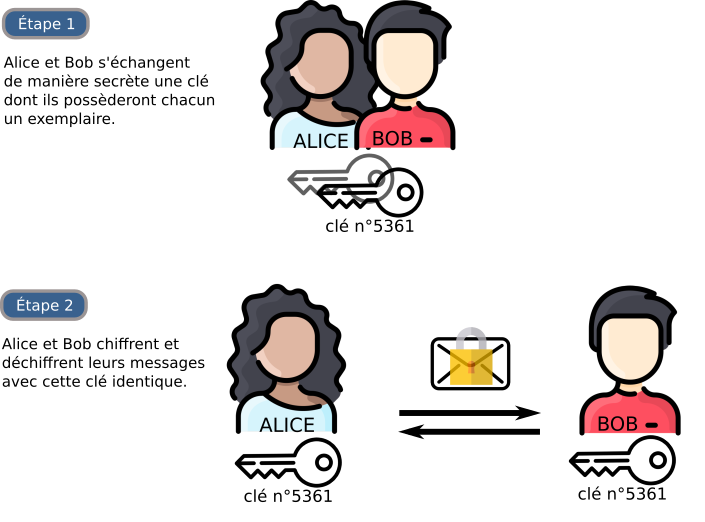
\includegraphics[height=160px]{sym.png}
		\end{center}
	\end{block}
\end{frame}

\begin{frame}
	\mframe{\SC}
	\begin{block}{Représentation du chiffrement asymétrique}
		\begin{center}
		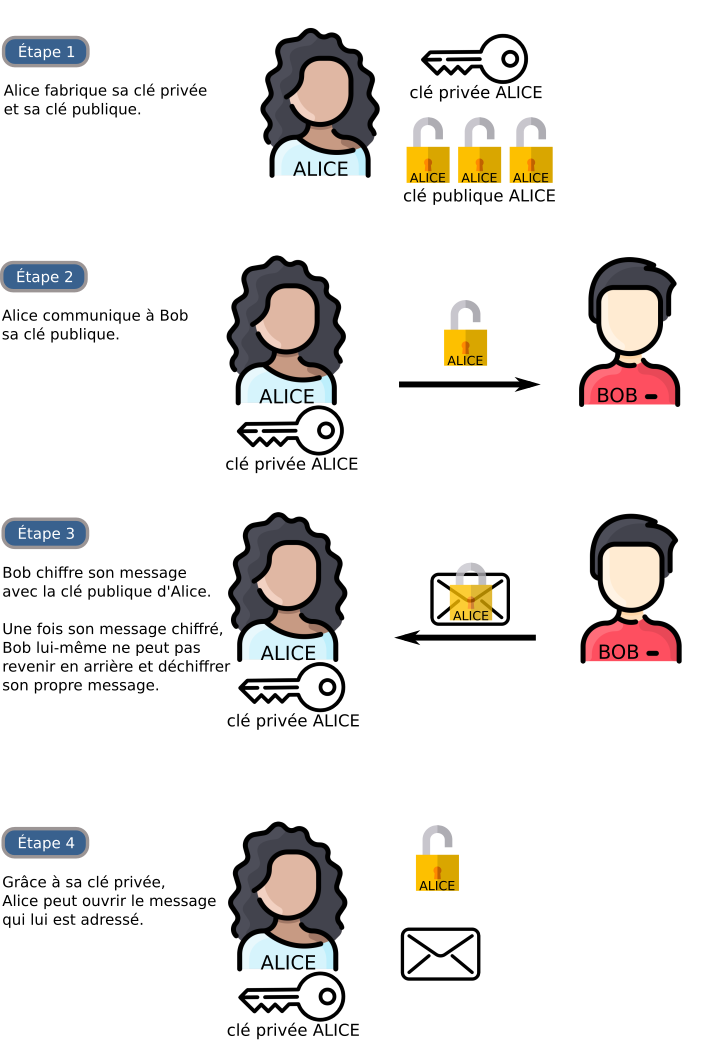
\includegraphics[height=160px]{asym.png}
		\end{center}
	\end{block}
\end{frame}


\begin{frame}
	\mframe{\SC}
	\begin{exampleblock}{Exemples}
		\begin{itemize}[label=\textbullet]
		\item<1-> Le code de César est l'un des premiers exemples historique :
		\begin{itemize}[label=\textbullet]
			\item<2-> La clé de chiffrement est un entier note $C$, par exemple 3.
			\item<3-> L'algorithme de chiffrement consiste alors à décaler chaque lettre de $C$ emplacements à droite dans l'alphabet. Avec une clé de 3, le message "NSI", se transforme  en "QVL".
			\item<4-> Pour déchiffrer on décale de $C$ emplacements à gauche.
			\item<5-> La connaissance des deux clés doit rester secrète, c'est donc un chiffrement symétrique.
		\end{itemize}
		\item<6-> Parmi les méthodes modernes (et bien plus robustes) de chiffrement symétrique, on peut citer : \textcolor{blue}{AES (Advanced Encryption Standard)} ou encore \textcolor{blue}{Chacha20}.
		\item<7-> L'exemple classique de chiffrement asymétrique est \textcolor{blue}{RSA} (voir activité.)
	\end{itemize}
	\end{exampleblock}
\end{frame}


\begin{frame}
	\mframe{\SC}
	\begin{block}{Avantages et inconvénients des deux méthodes}
		\begin{itemize}[label=\textbullet]
			\item<1-> Un chiffrement symétrique est souvent rapide et donc adapté au transfert d'un volume important d'informations.
			\item<2-> Un chiffrement symétrique peut-être très sûr (voire inviolable).\\
					\onslide<3->{\textcolor{OliveGreen}{\small Par exemple, un chiffrement {\sc xor} utilisant un masque aussi long que le message est inviolable}}
			\item<3-> L'inconvénient est que puisque le canal de transmission n'est pas sûr, les deux interlocuteurs doivent convenir \textcolor{blue}{au préalable} d'une clé de chiffrement.
			\item<4-> Dans un chiffrement asymétrique par contre, la clé de chiffrement peut être connue de tous car elle ne permet pas de déchiffrer. Elle peut donc être rendue publique sans mettre en danger la sécurité de la communication.
			\item<5-> Par contre, un chiffrement asymétrique peut être gourmand en ressource et donc non adapté à un volume important d'informations.
		\end{itemize}
	\end{block}
\end{frame}

\begin{frame}
	\mframe{\SC}
	\begin{block}{Protocole {\sc https}}
		Le protocole {\sc https} qui permet de sécuriser les transmissions est un exemple d'utilisation conjointe des deux méthodes : asymétrique et symétrique.
		\begin{center}
			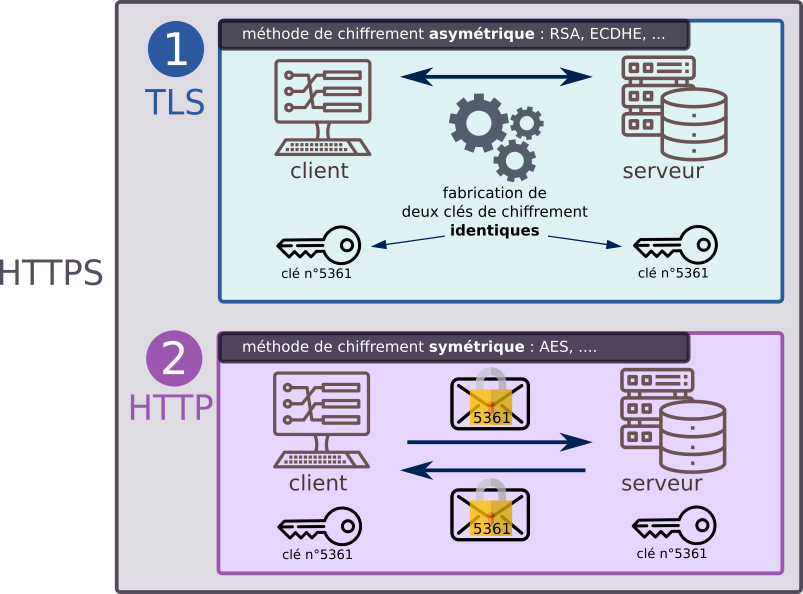
\includegraphics[height=160px]{https.png}
		\end{center}
	\end{block}
\end{frame}

\begin{frame}
	\mframe{\SC}
	\begin{block}{Autorité de certification}
		D'autre part, afin d'éviter une attaque du type \textit{homme du milieu} une autorité extérieure garanti l'identité du serveur.
		\begin{center}
			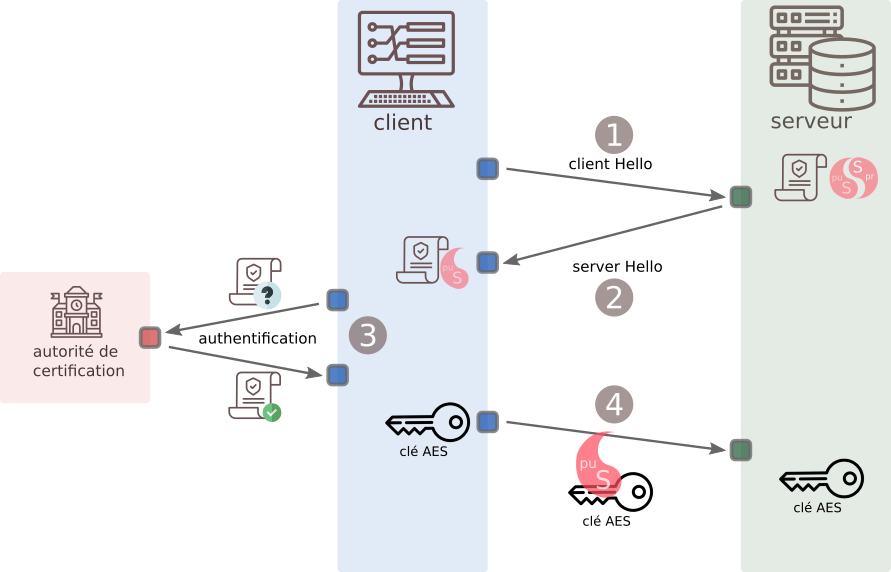
\includegraphics[height=160px]{tls.png}
		\end{center}
	\end{block}
\end{frame}

\end{document}